\chapter{Alte tehnologii folosite în aplicație}

\section{Bootstrap}

\emph{Boostrap}\footnote{\url{http://getbootstrap.com}}, 
dezvoltat inițial de Mark Otto 
și Jacob Thornton la Twitter, este un framework ce simplifică stilizarea
elementelor HTML cum ar fi form-uri și butoane și crearea
de meniuri de navigație, casete modale etc. De asemenea,
o parte foarte importantă a framework-ului este crearea aplicațiilor
\emph{responsive}, ceea ce înseamnă că aplicația este afișată
corect pe dispozitive cu display-uri de dimensiuni diferite:
calculatoare, tablete și telefoane.

Folosirea framework-ului este destul de simplă. Este
suficient să fie adăugate două fișiere din Bootstrap,
apoi clasele CSS pot fi folosite pentru stilizarea
elementelor HTML.


\section{Bower}

\emph{Bower}\footnote{\url{http://bower.io}} este o unealtă
folosită pentru managementul dependențelor de pe front-end.
Bower folosește fișierul \texttt{bower.json} pentru a 
ști ce trebuie să instaleze.

\lstinputlisting[title=app/bower.json]{chap4-code/bower.json}

Dependențele din \texttt{bower.json} sunt descărcate dintr-un
repository central în directorul \texttt{static/bower\_components}
cu comanda \texttt{bower install}.

\section{Git și GitHub}

\emph{Git}\footnote{https://git-scm.com} este un sistem distribuit
pentru controlul sistemului de reviziuni al fișierelor,
scris inițial de creatorul kernel-ului Linux, Linus Torvalds.
GitHub\footnote{http://github.com} este un serviciu
online ce permite găzduirea repository-urilor Git.

Atât codul aplicației, cât și codul aceastei lucrări, redactată folosind \LaTeX{},
sunt găzduite pe GitHub la adresele \url{https://github.com/stefan-mihaila/money-keep}
și \url{https://github.com/stefan-mihaila/thesis}.

\section{API REST (Django REST Framework)}

REST\footnote{\url{https://en.wikipedia.org/wiki/Representational_state_transfer}} (Representational State Transfer)
este o modalitate
de comunicare între servicii HTTP. REST a venit ca o alternativă
la SOAP\footnote{\url{https://en.wikipedia.org/wiki/SOAP}} și 
WSDL\footnote{\url{https://en.wikipedia.org/wiki/Web\_Services\_Description\_Language}}. 

SOAP și WSDL au încercat să ușureze munca dezvoltatorilor 
construind abstractizări deasupra
arhitecturii HTTP. REST a adoptat o altă strategie:
a introdus conceptul de resurse și a folosit
metodele HTTP existente pentru a procesa aceste resurse.

Metodele HTTP sunt următoarele:
\begin{description}
\item [OPTIONS] este metoda HTTP ce oferă clientului
posibilitate de a afla ce operații sunt disponibile
pentru o resursă, sau ce capacități are serverul,
fără însă a modifica resursa respectivă.
\item [GET] este metoda HTTP ce oferă detaliile unei resurse.
Această metodă este sigură și idempotentă.
\item [HEAD] este o metodă care se comportă ca și GET, cu 
excepția că serverul nu răspunde cu un BODY la acest request,
ci întoarce doar HEADER-ele HTTP.
\item [POST] este metoda HTTP ce creează o resursă nouă.
Serverul trebuie să răspundă cu 201 (Created) atunci când resursa
a fost creată cu succes și răspunsul trebuie să conțină
headerul LOCATION cu URL-ul resursei nou creată.
\item [PUT] este metoda HTTP folosită pentru a edita
o resursă. Toate proprietățile resursei trebuie trimise
de client, iar serverul editează suprascrie proprietățile resursei.
În cazul în care totul a decurs bine, răspunsul serverului
trebuie să fie 204 (No Content).
\item [DELETE] este metoda HTTP ce șterge resursa de pe server.
\end{description}

Proprietăți metodelor HTTP sunt următoarele:
\begin{description}
\item [siguranța] Metodele GET și HEAD sunt considerate
sigure, deoarece ele nu au efecte secundare, cum este cazul
metodelor POST, PUT și DELETE.
\item [idempotența] Metodele GET, HEAD, PUT și DELETE sunt
idempotente, adică rezultatul este același indiferent
dacă ele sunt chemate o dată sau de mai multe ori.
\end{description}

REST se pretează foarte bine arhitecturilor client server.
În REST, se consideră că există o mapare între URL-uri
și resurse. Avantajul REST este legat de faptul că acesta folosește
arhitectura existentă HTTP. De exemplu, pentru că
se folosesc metodele HTTP standard, resursele accesate
prin metoda GET pot fi stocate pe CDN-uri pentru acces
rapid, pentru că răspunsul acestei metode poate fi cacheable.

Django REST Framework este un plugin de Django
ce permite crearea rapidă de resurse HTTP folosindu-se
modelele din Django. În plus, endpoint-urile acestui framework
oferă o interfață web ce ușurează debugging-ul și dezvoltarea
rapidă.

\begin{figure}[t]
  \centering
    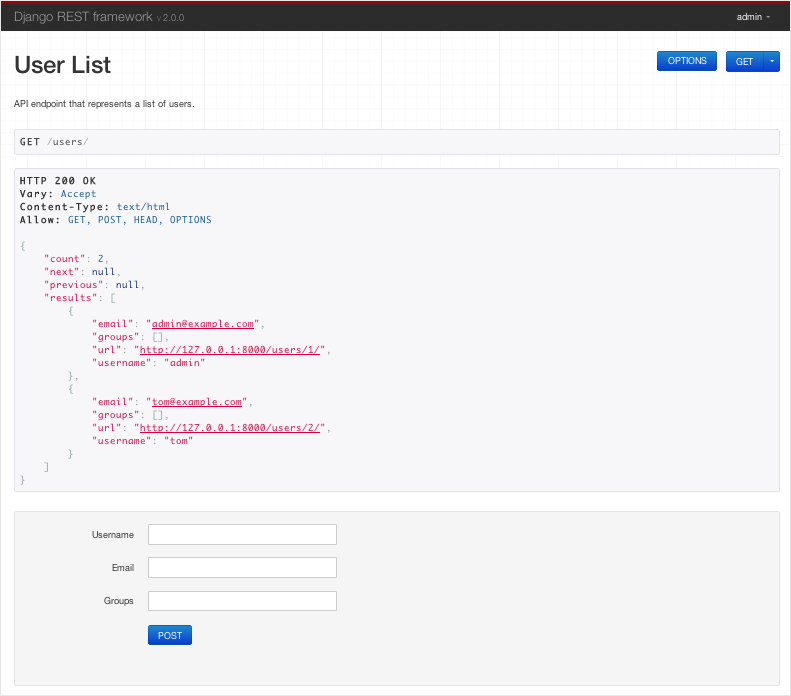
\includegraphics[width=1\textwidth]{./chap4-code/rest_framework}
  \caption{Interfață web REST Framework}
\end{figure}